% Name
有道搜索框

% Legend
在有道搜索框中,当输入一个或者多个字符时,搜索框会出现一定数量的提示,如下图所示:

\begin{center}
    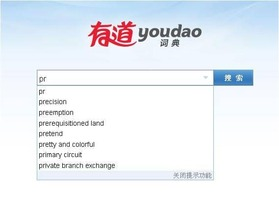
\includegraphics[bb=0 0 1000 1000]{youdao.jpg}
\end{center}

现在给你 $N$ 个单词和一些查询,请输出提示结果,为了简化这个问题,只需要输出以查询词为前缀的并且按字典序排列的最前面的 $8$ 个单词,如果符合要求的单词一个也没有请只输出当前查询词。

% Input format
第一行是一个正整数 $N$ ,表示词表中有 $N$ 个单词。

接下来有 $N$ 行,每行都有一个单词,注意词表中的单词可能有重复,请忽略掉重复单词。

接下来的一行有一个正整数 $Q$ ,表示接下来有 $Q$ 个查询。

接下来 $Q$ 行,每行有一个单词,表示一个查询词。

所有的单词和查询词都是由小写字母组成,并且所有的单词以及查询词的长度都不超过 20 ,且都不为空。

其中: $N \leq 10000, Q \leq 10000$

% Output format
对于每个查询,输出一行,按顺序输出该查询词的提示结果,用空格隔开。
